\begin{trapbox}
\begin{itemize}
  \item \textbf{把椭圆当圆：}一般不能把距离极值写成
  “点到中心距离 $\pm$ 半长轴/半短轴”。
  \item \textbf{把 $M$ 当作特殊点：}题中的 $M(x_0,y_0)$
  是任意外点，不要求在坐标轴上，也不要求是椭圆中心。
  \item \textbf{不检验外点条件：}本结论的题设为
  $\dfrac{x_0^2}{a^2}+\dfrac{y_0^2}{b^2}>1$；
  等号表示点在椭圆上，不能混同。
  \item \textbf{只找一个驻点：}导数等于零给的是
  极值\emph{候选点}；须比较所有候选点，才能确定全局最小和最大。
  \item \textbf{万能代换漏点：} $t=\tan(\theta/2)$
  没有覆盖 $\theta=\pi$；需检查 $P=(-a,0)$。
  \item \textbf{漏掉平方与开方：}先比较 $MP^2$，
  最终所求距离为非负平方根，而不是距离平方。
  \item \textbf{误认为极值一定在顶点：}一般外点的最近点、
  最远点不一定在长轴或短轴端点。
\end{itemize}

\medskip\textbf{法向量法特别提醒：}
\begin{itemize}
\item 法向量不是位置向量 $(x,y)$，而是 $(x/a^2,y/b^2)$；一般 $M,P,O$ 不共线。
\item $\lambda$ 不是距离；$MP=|\lambda|\sqrt{x^2/a^4+y^2/b^4}$。
\item 法线条件只是必要条件；最近点取唯一正根，最远点不能直接取任意负根。
\item 清分母不能忽略 $\lambda=-a^2,-b^2$，必须回原方程核对。
\end{itemize}
% C083: extracted shared teaching figure.
\begin{center}
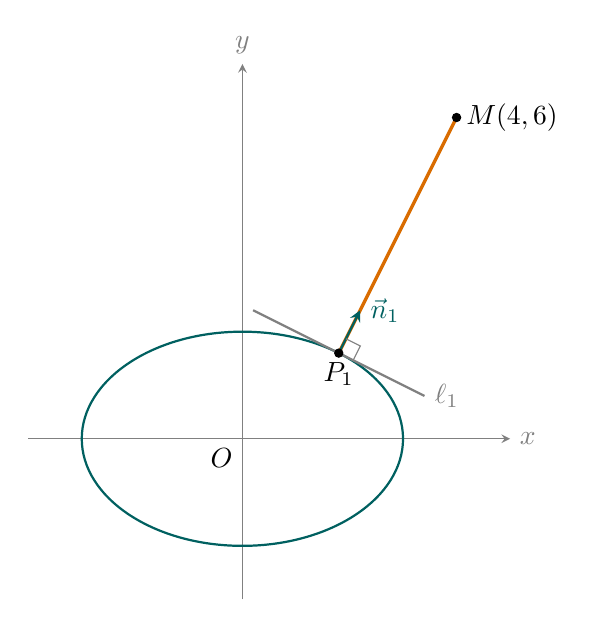
\begin{tikzpicture}[scale=.68,>=stealth]
\draw[->,gray] (-4,0)--(5,0) node[right]{$x$};
\draw[->,gray] (0,-3)--(0,7) node[above]{$y$};
\draw[teal!75!black,thick] (0,0) ellipse (3 and 2);
\coordinate (M) at (4,6); \coordinate (P) at (1.8,1.6);
\draw[orange!85!black,very thick] (P)--(M);
\draw[gray,thick] (.2,2.4)--(3.4,.8) node[right]{$\ell_1$};
\draw[->,teal!75!black,thick] (P)--(2.2,2.4) node[right]{$\vec n_1$};
\draw[gray] (2.068,1.466)--(2.202,1.734)--(1.934,1.868);
\fill (M) circle (2.5pt) node[right]{$M(4,6)$};
\fill (P) circle (2.5pt) node[below]{$P_1$};
\node[below left] at (0,0) {$O$};
\end{tikzpicture}
\end{center}


\end{trapbox}
